\chapter{Исследования}

\section{Предварительное описание}

Проведем сначала тестирование программы на работоспособность. Образец расчетной области изображен на рисунке \ref{fig:exampleOfArea}. Это область $\Omega = [1.0, 2.0]_r \times [1.0, 2.0]_z$, она содержит 16 узлов, а на всех границах будем задавать первые краевые условия.

\begin{figure}
	\centering
	\includegraphics[width=0.75\linewidth]{images/"3D_grid_example".png}
	\caption{Расчетная область}
	\label{fig:exampleOf3DMesh}
\end{figure}

\section{Тестирование на порядок аппроксимации}

\begin{table}
	\caption{Тестирование при $u = 2$, $f = \frac{2}{r^2}$, $\mu_0 = 1$}
	\centering
	\small
	\begin{tabularx}{1.0\textwidth}{| >{\raggedright\arraybackslash}X | >{\raggedright\arraybackslash}X | >{\raggedright\arraybackslash}X |>{\raggedright\arraybackslash}X |}
		\hline
		\centering{Узел} & \centering{Значение} & \centering{Абсолютная погрешность} & \centering{Относительная погрешность} \tabularnewline \hline
		
	

		 \centering{(${}^4/_3$; ${}^4/_3$)} & \centering{2.00226896E+000}& \centering{2.26896083E-003} & \centering{1.13448042E-003} \tabularnewline \hline
		 
		 \centering{(${}^5/_3$; ${}^4/_3$)} & \centering{2.00130487E+000} & \centering{1.30486533E-003} & \centering{6.52432666E-004} \tabularnewline \hline
  		 
  		 \centering{(${}^4/_3$; ${}^5/_3$)} & \centering{2.00226896E+000} & \centering{2.26896083E-003} & \centering{1.13448042E-003} \tabularnewline \hline
		 
		 \centering{(${}^5/_3$; ${}^5/_3$)} & \centering{2.00130487E+000} & \centering{1.30486533E-003} & \centering{6.52432666E-004} \tabularnewline \hline
		 
 	\end{tabularx}
	\label{tab:test1}
\end{table}

\begin{table}
	\caption{Тестирование при $u = r$, $f = 0$, $\mu_0 = 1$}
	\centering
	\small
	\begin{tabularx}{1.0\textwidth}{| >{\raggedright\arraybackslash}X | >{\raggedright\arraybackslash}X | >{\raggedright\arraybackslash}X |>{\raggedright\arraybackslash}X |}
		\hline
		\centering{Узел} & \centering{Значение} & \centering{Абсолютная погрешность} & \centering{Относительная погрешность} \tabularnewline \hline
		
		
		
		\centering{(${}^4/_3$; ${}^4/_3$)} & \centering{1.33333333E+000}& \centering{1.33226763E-015} & \centering{9.99200722E-016} \tabularnewline \hline
		
		\centering{(${}^5/_3$; ${}^4/_3$)} & \centering{1.66666667E+000} & \centering{6.66133815E-016} & \centering{3.99680289E-016} \tabularnewline \hline
		
		\centering{(${}^4/_3$; ${}^5/_3$)} & \centering{1.33333333E+000} & \centering{1.77635684E-015} & \centering{1.33226763E-015} \tabularnewline \hline
		
		\centering{(${}^5/_3$; ${}^5/_3$)} & \centering{1.66666667E+000} & \centering{6.66133815E-016} & \centering{3.99680289E-016} \tabularnewline \hline
		
	\end{tabularx}
	\label{tab:test2}
\end{table}

\begin{table}
\caption{Тестирование при $u = z$, $f = \frac{z}{r^2}$, $\mu_0 = 1$}
\centering
\small
\begin{tabularx}{1.0\textwidth}{| >{\raggedright\arraybackslash}X | >{\raggedright\arraybackslash}X | >{\raggedright\arraybackslash}X |>{\raggedright\arraybackslash}X |}
	\hline
	\centering{Узел} & \centering{Значение} & \centering{Абсолютная погрешность} & \centering{Относительная погрешность} \tabularnewline \hline
	
	
	
	\centering{(${}^4/_3$; ${}^4/_3$)} & \centering{1.33491362E+000}& \centering{1.58028263E-003} & \centering{1.18521198E-003} \tabularnewline \hline
	
	\centering{(${}^5/_3$; ${}^4/_3$)} & \centering{1.33426439E+000} & \centering{9.31054340E-004} & \centering{6.98290755E-004} \tabularnewline \hline
	
	\centering{(${}^4/_3$; ${}^5/_3$)} & \centering{1.66848983E+000} & \centering{1.82315862E-003} & \centering{1.09389517E-003} \tabularnewline \hline
	
	\centering{(${}^5/_3$; ${}^5/_3$)} & \centering{1.66769291E+000} & \centering{1.02624366E-003} & \centering{6.15746195E-004} \tabularnewline \hline
	
\end{tabularx}
\label{tab:test3}
\end{table}

\begin{table}
\caption{Тестирование при $u = r+z$, $f = \frac{z}{r^2}$, $\mu_0 = 1$}
\centering
\small
\begin{tabularx}{1.0\textwidth}{| >{\raggedright\arraybackslash}X | >{\raggedright\arraybackslash}X | >{\raggedright\arraybackslash}X |>{\raggedright\arraybackslash}X |}
	\hline
	\centering{Узел} & \centering{Значение} & \centering{Абсолютная погрешность} & \centering{Относительная погрешность} \tabularnewline \hline
	
	
	
	\centering{(${}^4/_3$; ${}^4/_3$)} & \centering{2.66824695E+000}& \centering{1.58028263E-003} & \centering{5.92605988E-004} \tabularnewline \hline
	
	\centering{(${}^5/_3$; ${}^4/_3$)} & \centering{3.00093105E+000} & \centering{9.31054340E-004} & \centering{3.10351447E-004} \tabularnewline \hline
	
	\centering{(${}^4/_3$; ${}^5/_3$)} & \centering{3.00182316E+000} & \centering{1.82315862E-003} & \centering{6.07719539E-004} \tabularnewline \hline
	
	\centering{(${}^5/_3$; ${}^5/_3$)} & \centering{3.33435958E+000} & \centering{1.02624366E-003} & \centering{3.07873097E-004} \tabularnewline \hline
	
\end{tabularx}
\label{tab:test4}
\end{table}

\begin{table}
\caption{Тестирование при $u = rz$, $f = 0$, $\mu_0 = 1$}
\centering
\small
\begin{tabularx}{1.0\textwidth}{| >{\raggedright\arraybackslash}X | >{\raggedright\arraybackslash}X | >{\raggedright\arraybackslash}X |>{\raggedright\arraybackslash}X |}
	\hline
	\centering{Узел} & \centering{Значение} & \centering{Абсолютная погрешность} & \centering{Относительная погрешность} \tabularnewline \hline
	
	
	
	\centering{(${}^4/_3$; ${}^4/_3$)} & \centering{1.77777778E+000}& \centering{1.11022302E-015} & \centering{6.24500451E-016} \tabularnewline \hline
	
	\centering{(${}^5/_3$; ${}^4/_3$)} & \centering{2.22222222E+000} & \centering{3.10862447E-015} & \centering{1.39888101E-015} \tabularnewline \hline
	
	\centering{(${}^4/_3$; ${}^5/_3$)} & \centering{2.22222222E+000} & \centering{8.88178420E-016} & \centering{3.99680289E-016} \tabularnewline \hline
	
	\centering{(${}^5/_3$; ${}^5/_3$)} & \centering{2.77777778E+000} & \centering{4.88498131E-015} & \centering{1.75859327E-015} \tabularnewline \hline
	
\end{tabularx}
\label{tab:test5}
\end{table}

\begin{table}
\caption{Тестирование при $u = r^2 + z^2$, $f = \frac{z^2}{r^2} - 5$, $\mu_0 = 1$}
\centering
\small
\begin{tabularx}{1.0\textwidth}{| >{\raggedright\arraybackslash}X | >{\raggedright\arraybackslash}X | >{\raggedright\arraybackslash}X |>{\raggedright\arraybackslash}X |}
	\hline
	\centering{Узел} & \centering{Значение} & \centering{Абсолютная погрешность} & \centering{Относительная погрешность} \tabularnewline \hline
	
	
	
	\centering{(${}^4/_3$; ${}^4/_3$)} & \centering{3.55717205E+000}& \centering{1.61649660E-003} & \centering{4.54639669E-004} \tabularnewline \hline
	
	\centering{(${}^5/_3$; ${}^4/_3$)} & \centering{4.55644336E+000} & \centering{8.87803368E-004} & \centering{1.94883666E-004} \tabularnewline \hline
	
	\centering{(${}^4/_3$; ${}^5/_3$)} & \centering{4.55790068E+000} & \centering{2.34512455E-003} & \centering{5.14783438E-004} \tabularnewline \hline
	
	\centering{(${}^5/_3$; ${}^5/_3$)} & \centering{5.55672893E+000} & \centering{1.17337132E-003} & \centering{2.11206838E-004} \tabularnewline \hline
	
\end{tabularx}
\label{tab:test6}
\end{table}

\begin{table}
\caption{Тестирование при $u = r^2 z^2$, $f = -3z^2 - 2r^2$, $\mu_0 = 1$}
\centering
\small
\begin{tabularx}{1.0\textwidth}{| >{\raggedright\arraybackslash}X | >{\raggedright\arraybackslash}X | >{\raggedright\arraybackslash}X |>{\raggedright\arraybackslash}X |}
	\hline
	\centering{Узел} & \centering{Значение} & \centering{Абсолютная погрешность} & \centering{Относительная погрешность} \tabularnewline \hline
	
	
	
	\centering{(${}^4/_3$; ${}^4/_3$)} & \centering{3.15919390E+000}& \centering{1.29993140E-003} & \centering{4.11306418E-004} \tabularnewline \hline
	
	\centering{(${}^5/_3$; ${}^4/_3$)} & \centering{4.93728492E+000} & \centering{9.86688136E-004} & \centering{1.99804348E-004} \tabularnewline \hline
	
	\centering{(${}^4/_3$; ${}^5/_3$)} & \centering{4.93658403E+000} & \centering{1.68757555E-003} & \centering{3.41734049E-004} \tabularnewline \hline
	
	\centering{(${}^5/_3$; ${}^5/_3$)} & \centering{7.71481536E+000} & \centering{1.23402231E-003} & \centering{1.59929291E-004} \tabularnewline \hline
	
\end{tabularx}
\label{tab:test7}
\end{table}

\begin{table}
\caption{Тестирование при $u = r^3+z^3$, $f = -8r -6z + \frac{z^3}{r^2}$, $\mu_0 = 1$}
\centering
\small
\begin{tabularx}{1.0\textwidth}{| >{\raggedright\arraybackslash}X | >{\raggedright\arraybackslash}X | >{\raggedright\arraybackslash}X |>{\raggedright\arraybackslash}X |}
	\hline
	\centering{Узел} & \centering{Значение} & \centering{Абсолютная погрешность} & \centering{Относительная погрешность} \tabularnewline \hline
	
	
	
	\centering{(${}^4/_3$; ${}^4/_3$)} & \centering{4.73874864E+000}& \centering{1.99210278E-003} & \centering{4.20209180E-004} \tabularnewline \hline
	
	\centering{(${}^5/_3$; ${}^4/_3$)} & \centering{6.99757994E+000} & \centering{2.42006018E-003} & \centering{3.45722883E-004} \tabularnewline \hline
	
	\centering{(${}^4/_3$; ${}^5/_3$)} & \centering{6.99968104E+000} & \centering{3.18957115E-004} & \centering{4.55653022E-005} \tabularnewline \hline
	
	\centering{(${}^5/_3$; ${}^5/_3$)} & \centering{9.25749495E+000} & \centering{1.76431155E-003} & \centering{1.90545647E-004} \tabularnewline \hline
	
\end{tabularx}
\label{tab:test8}
\end{table}

\begin{table}
\caption{Тестирование при $u = r^3 z^3$, $f = -8rz^3 - 6r^3 z$, $\mu_0 = 1$}
\centering
\small
\begin{tabularx}{1.0\textwidth}{| >{\raggedright\arraybackslash}X | >{\raggedright\arraybackslash}X | >{\raggedright\arraybackslash}X |>{\raggedright\arraybackslash}X |}
	\hline
	\centering{Узел} & \centering{Значение} & \centering{Абсолютная погрешность} & \centering{Относительная погрешность} \tabularnewline \hline
	
	
	
	\centering{(${}^4/_3$; ${}^4/_3$)} & \centering{5.60268110E+000}& \centering{1.59745896E-002} & \centering{2.84313374E-003} \tabularnewline \hline
	
	\centering{(${}^5/_3$; ${}^4/_3$)} & \centering{1.09603120E+001} & \centering{1.36249123E-002} & \centering{1.24157014E-003} \tabularnewline \hline
	
	\centering{(${}^4/_3$; ${}^5/_3$)} & \centering{1.09509327E+001} & \centering{2.30042146E-002} & \centering{2.09625906E-003} \tabularnewline \hline
	
	\centering{(${}^5/_3$; ${}^5/_3$)} & \centering{2.14142095E+001} & \centering{1.92609735E-002} & \centering{8.98639979E-004} \tabularnewline \hline
	
\end{tabularx}
\label{tab:test9}
\end{table}

Исходя из полученных данных, можно сказать, что программа верно находит численное решение задачи.

\section{Тестирование на порядок сходимости}

Рассмотрим решение функции $u = r^3 + z^3$, последовательно разбивая сетку в 2 раза. 

\begin{table}
	\caption{Тестирование при $u = r^3 + z^3$, $f = -8rz^3 - 6r^3 z$, $\mu_0 = 1$}
	\centering
	\small
	\begin{tabularx}{1.0\textwidth}{| >{\raggedright\arraybackslash}X | >{\raggedright\arraybackslash}X | >{\raggedright\arraybackslash}X |>{\raggedright\arraybackslash}X |}
		\hline
		\centering{Количество разбиений} & \centering{Средняя погрешность} & \centering{Порядок сходимости} \tabularnewline \hline		
		
		\centering{2} & \centering{1.7116567E-004}& \centering{-} \tabularnewline \hline
		
		\centering{4} & \centering{5.2066366E-005} & \centering{1.716969754} \tabularnewline \hline
		
		\centering{8} & \centering{1.4089198E-005} & \centering{1.885762274} \tabularnewline \hline
		
		\centering{16} & \centering{3.6602112E-006} & \centering{1.94459064} \tabularnewline \hline
		
		\centering{32} & \centering{9.3301457E-007} & \centering{1.971955381} \tabularnewline \hline
		
	\end{tabularx}
	\label{tab:test11}
\end{table}

Порядок сходимости стремится к 2.

\section{Тестирование первичного поля}

Пусть имеется рассчетная область $\Omega = [0.001; 125.0]_r \times [-80.0; 0.0]_z$. Источник поля лежит на расстоянии $R = 10$ от начала координат и имееет силу тока, равную $J_{\varphi} = 1.0$. Источник работал достаточно долго, чтобы создать стабильное электромагнитное поле. Сетка по времени: $t=[0.0; 60.0]$. Пусть после первой секунды мы отключим наш источник, т.е. $J_{\varphi} = 0.0$ при $t > 1.0$.

\begin{figure}
	\centering
	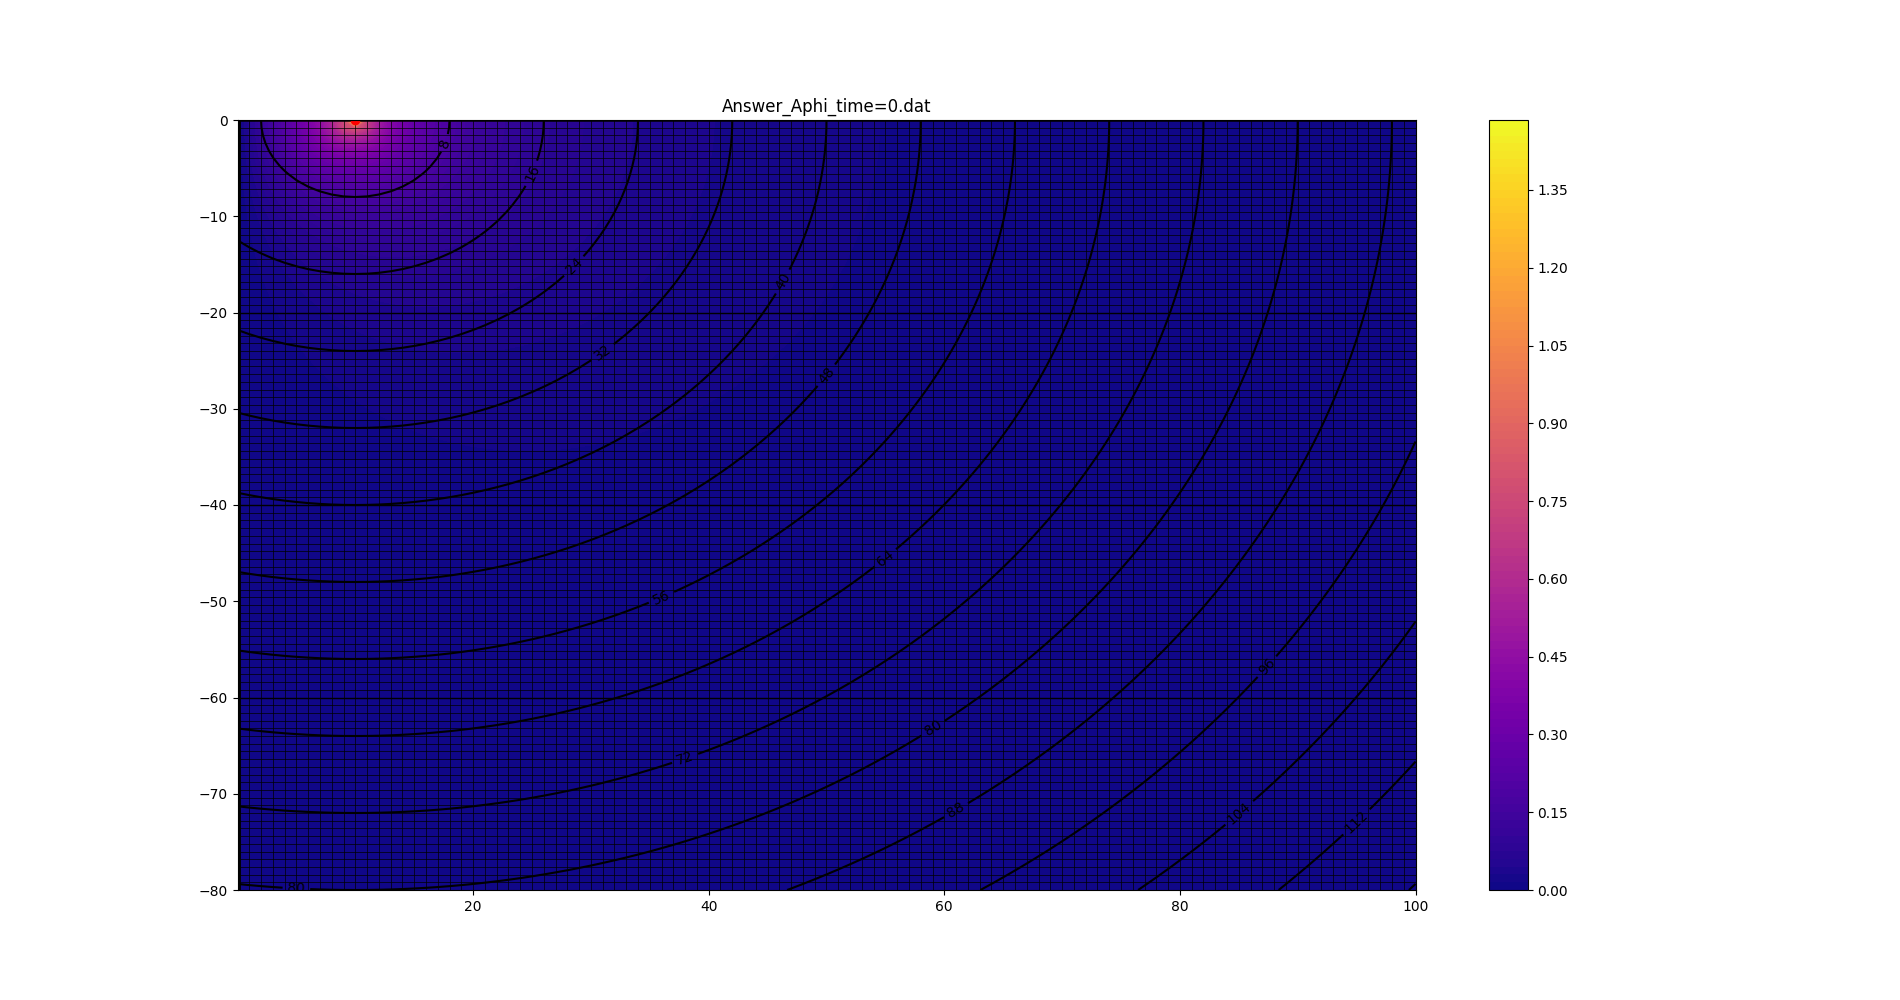
\includegraphics[width=0.9\linewidth]{images/Answer_Aphi_time=0.png}
	\caption{Решение $A_{\varphi}(r, z, 0.0)$}
	\label{fig:A_phi_0}
\end{figure}

\begin{figure}
	\centering
	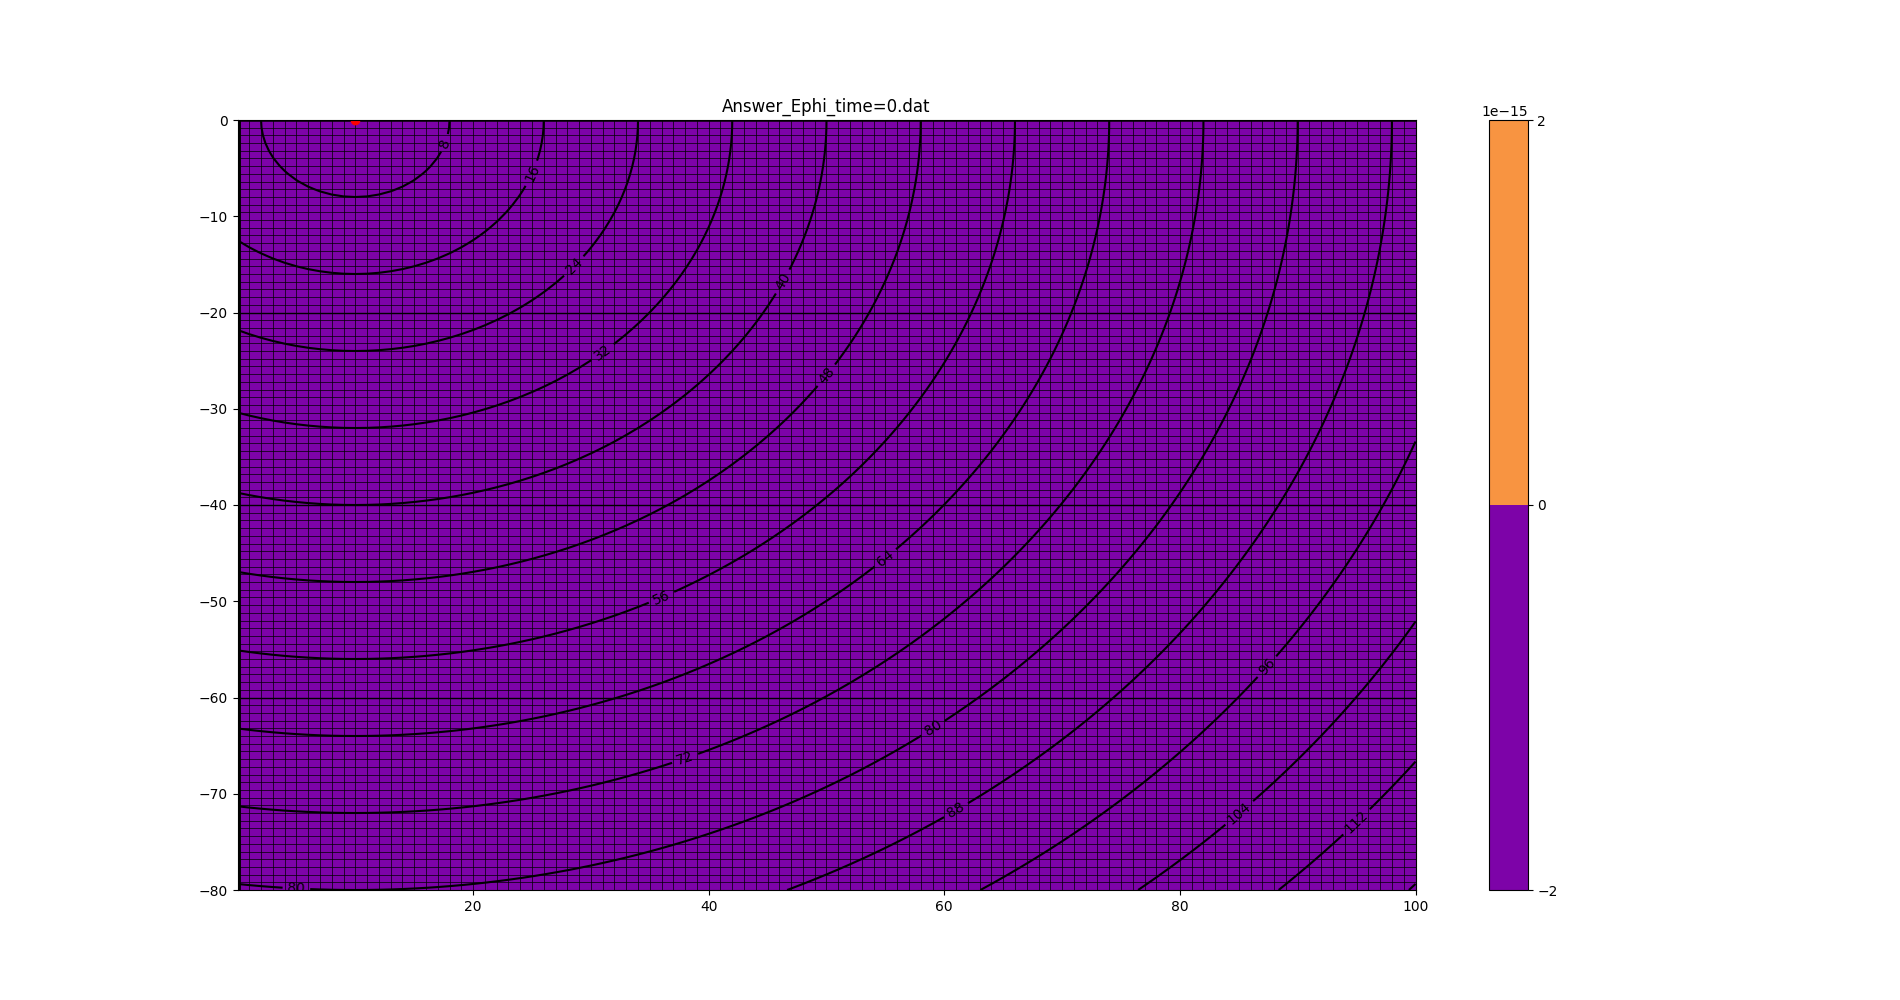
\includegraphics[width=0.9\linewidth]{images/Answer_Ephi_time=0.png}
	\caption{Решение $E_{\varphi}(r, z, 0.0)$}
	\label{fig:E_phi_0}
\end{figure}

\begin{figure}
	\centering
	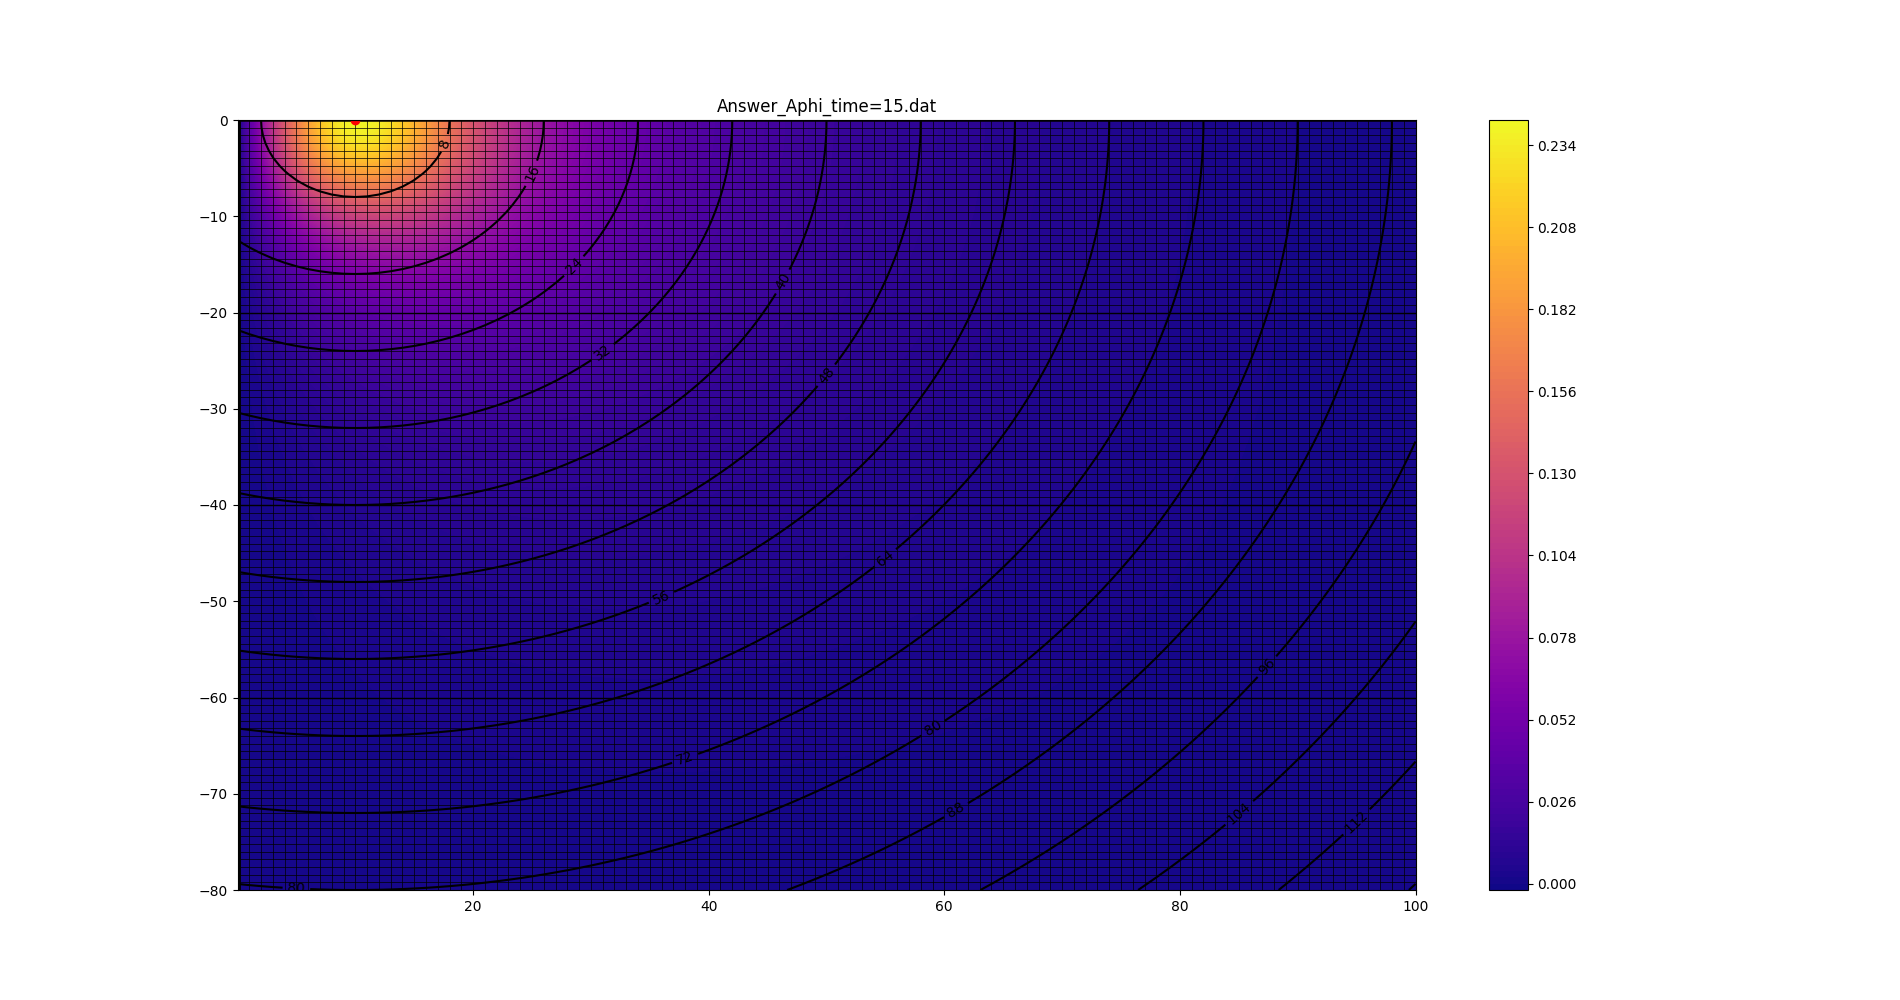
\includegraphics[width=1.0\linewidth]{images/Answer_Aphi_time=15.png}
	\caption{Решение $A_{\varphi}(r, z, 15.0)$}
	\label{fig:A_phi_15}
\end{figure}

\begin{figure}
	\centering
	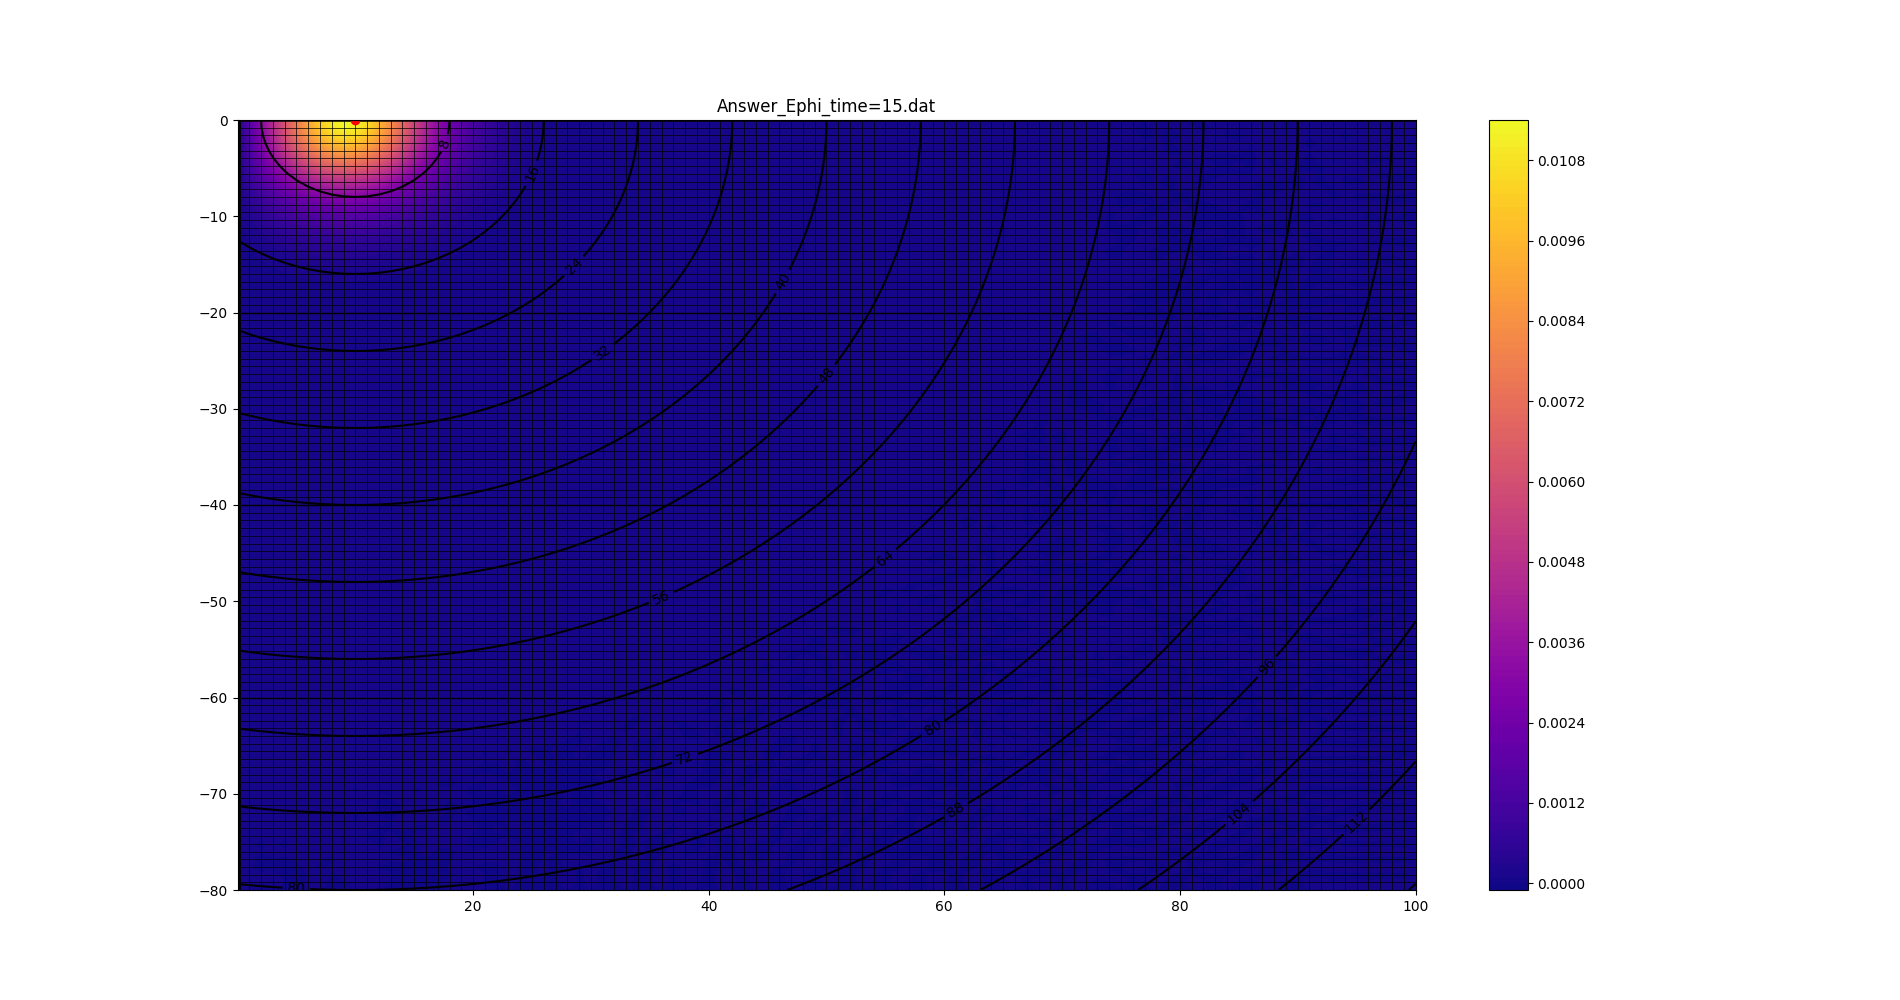
\includegraphics[width=1.0\linewidth]{images/Answer_Ephi_time=15.png}
	\caption{Решение $A_{\varphi}(r, z, 15.0)$}
	\label{fig:E_phi_15}
\end{figure} 

\begin{figure}
	\centering
	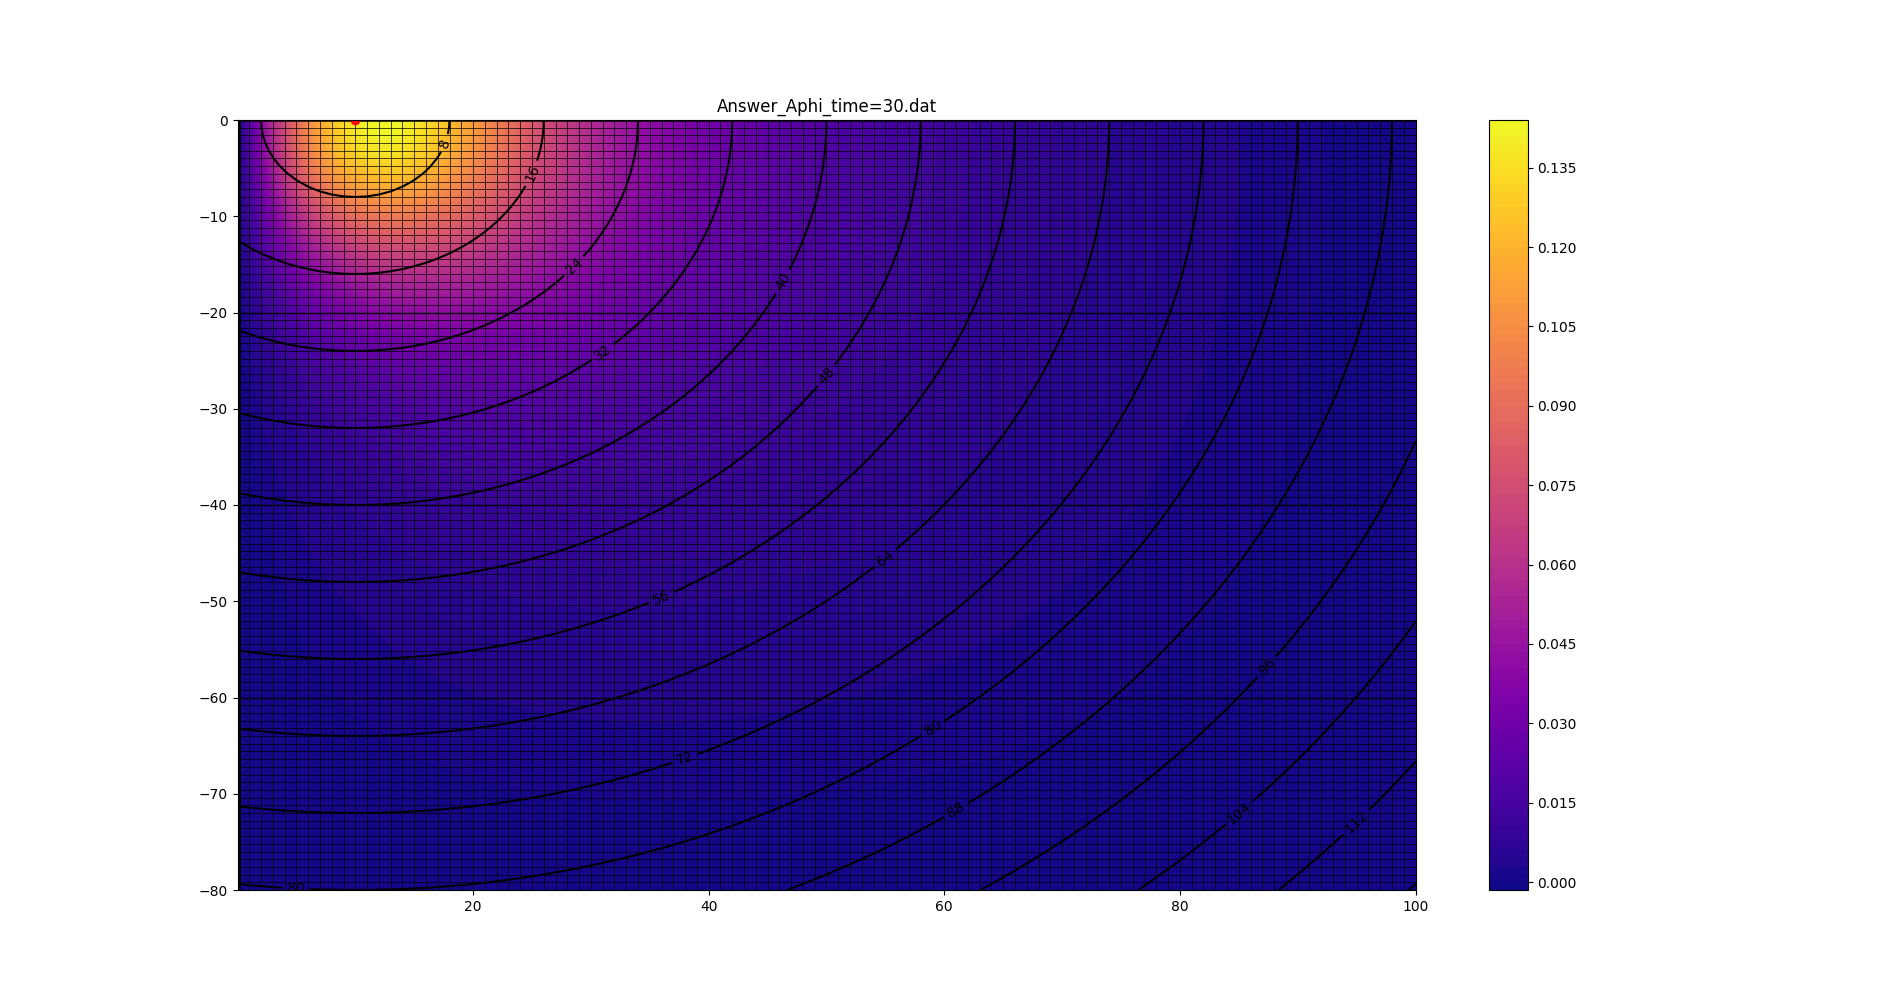
\includegraphics[width=1.0\linewidth]{images/Answer_Aphi_time=30.png}
	\caption{Решение $A_{\varphi}(r, z, 30.0)$}
	\label{fig:A_phi_30}
\end{figure}

\begin{figure}
	\centering
	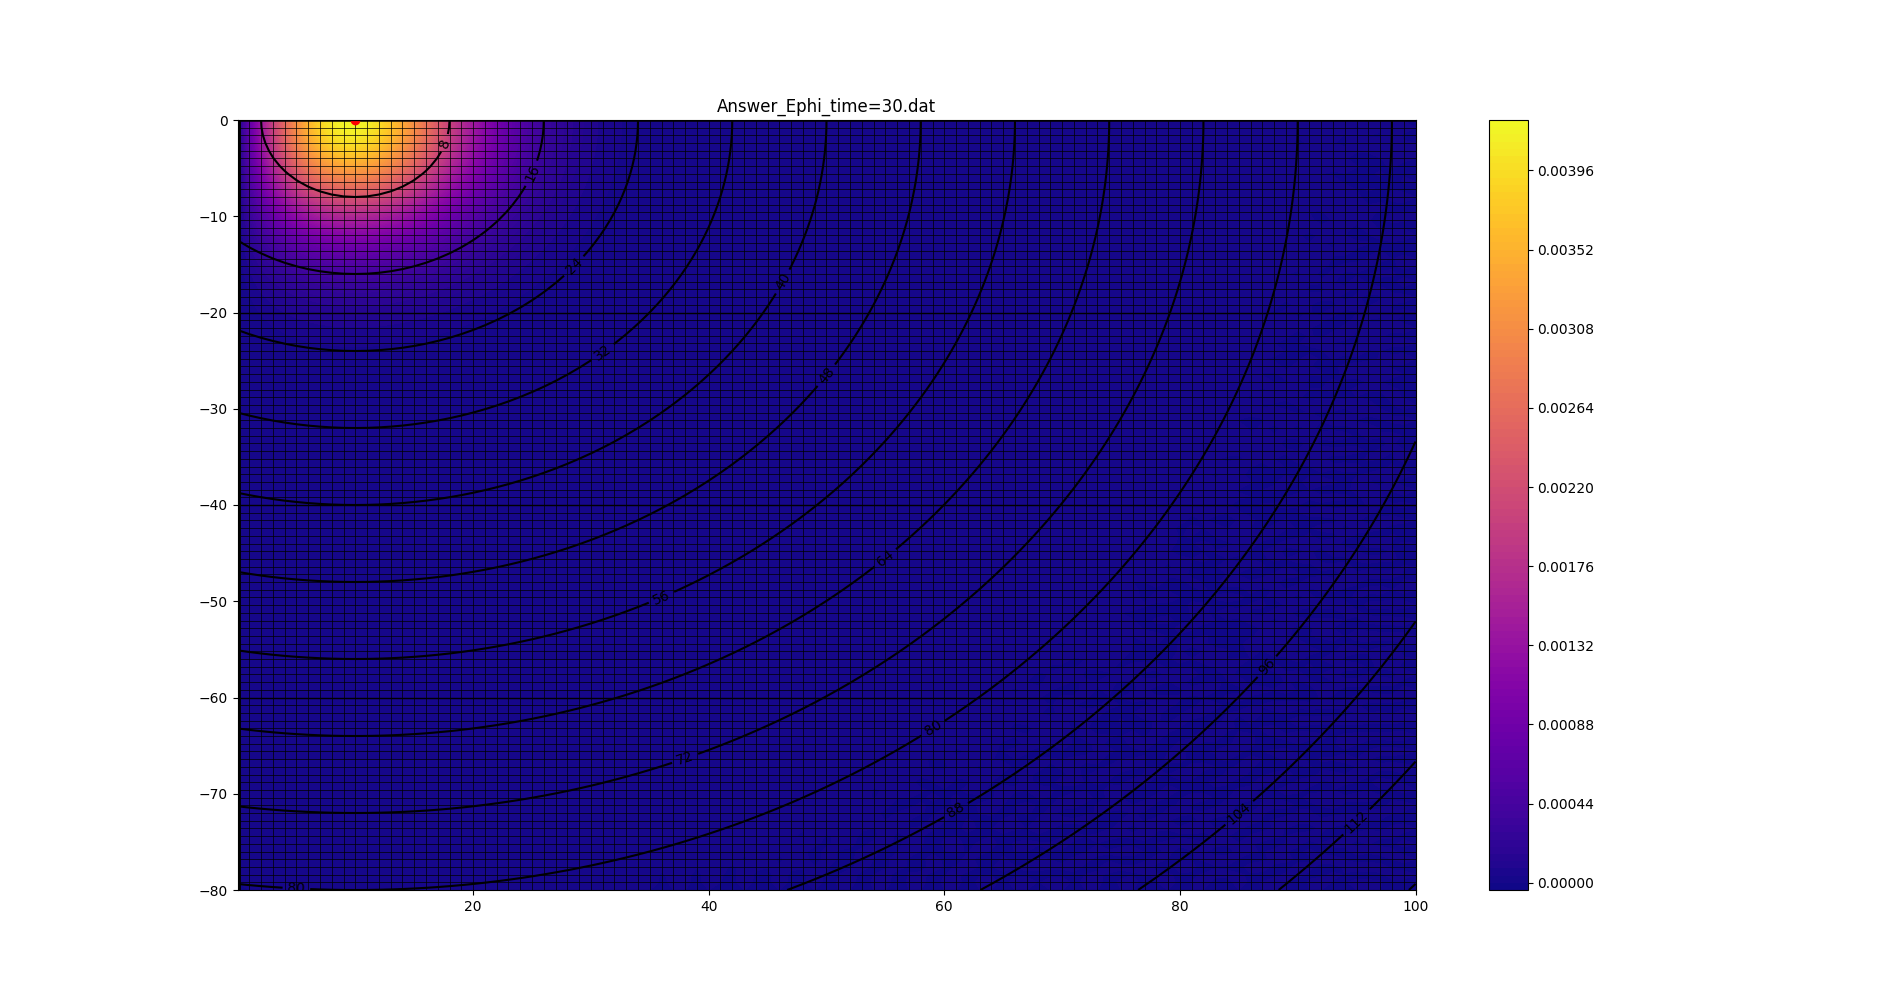
\includegraphics[width=1.0\linewidth]{images/Answer_Ephi_time=30.png}
	\caption{Решение $A_{\varphi}(r, z, 30.0)$}
	\label{fig:E_phi_30}
\end{figure} 

\begin{figure}
	\centering
	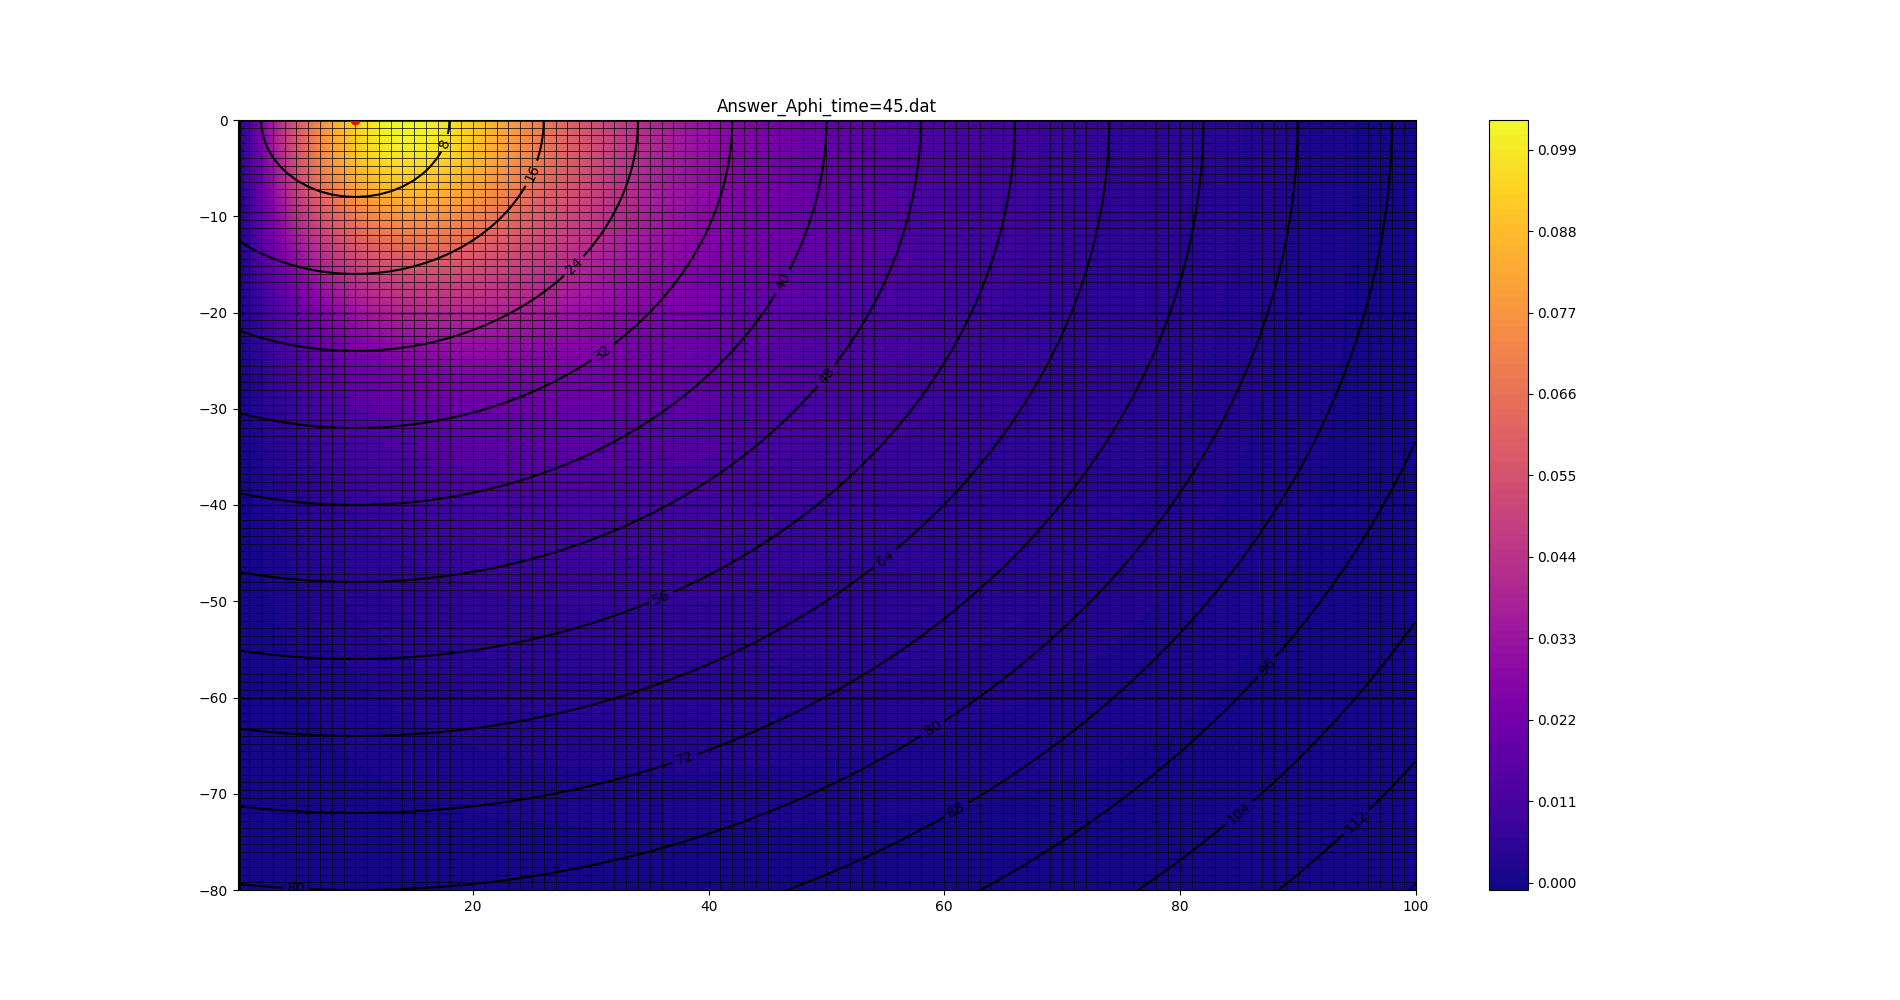
\includegraphics[width=1.0\linewidth]{images/Answer_Aphi_time=45.png}
	\caption{Решение $A_{\varphi}(r, z, 45.0)$}
	\label{fig:A_phi_45}
\end{figure}

\begin{figure}
	\centering
	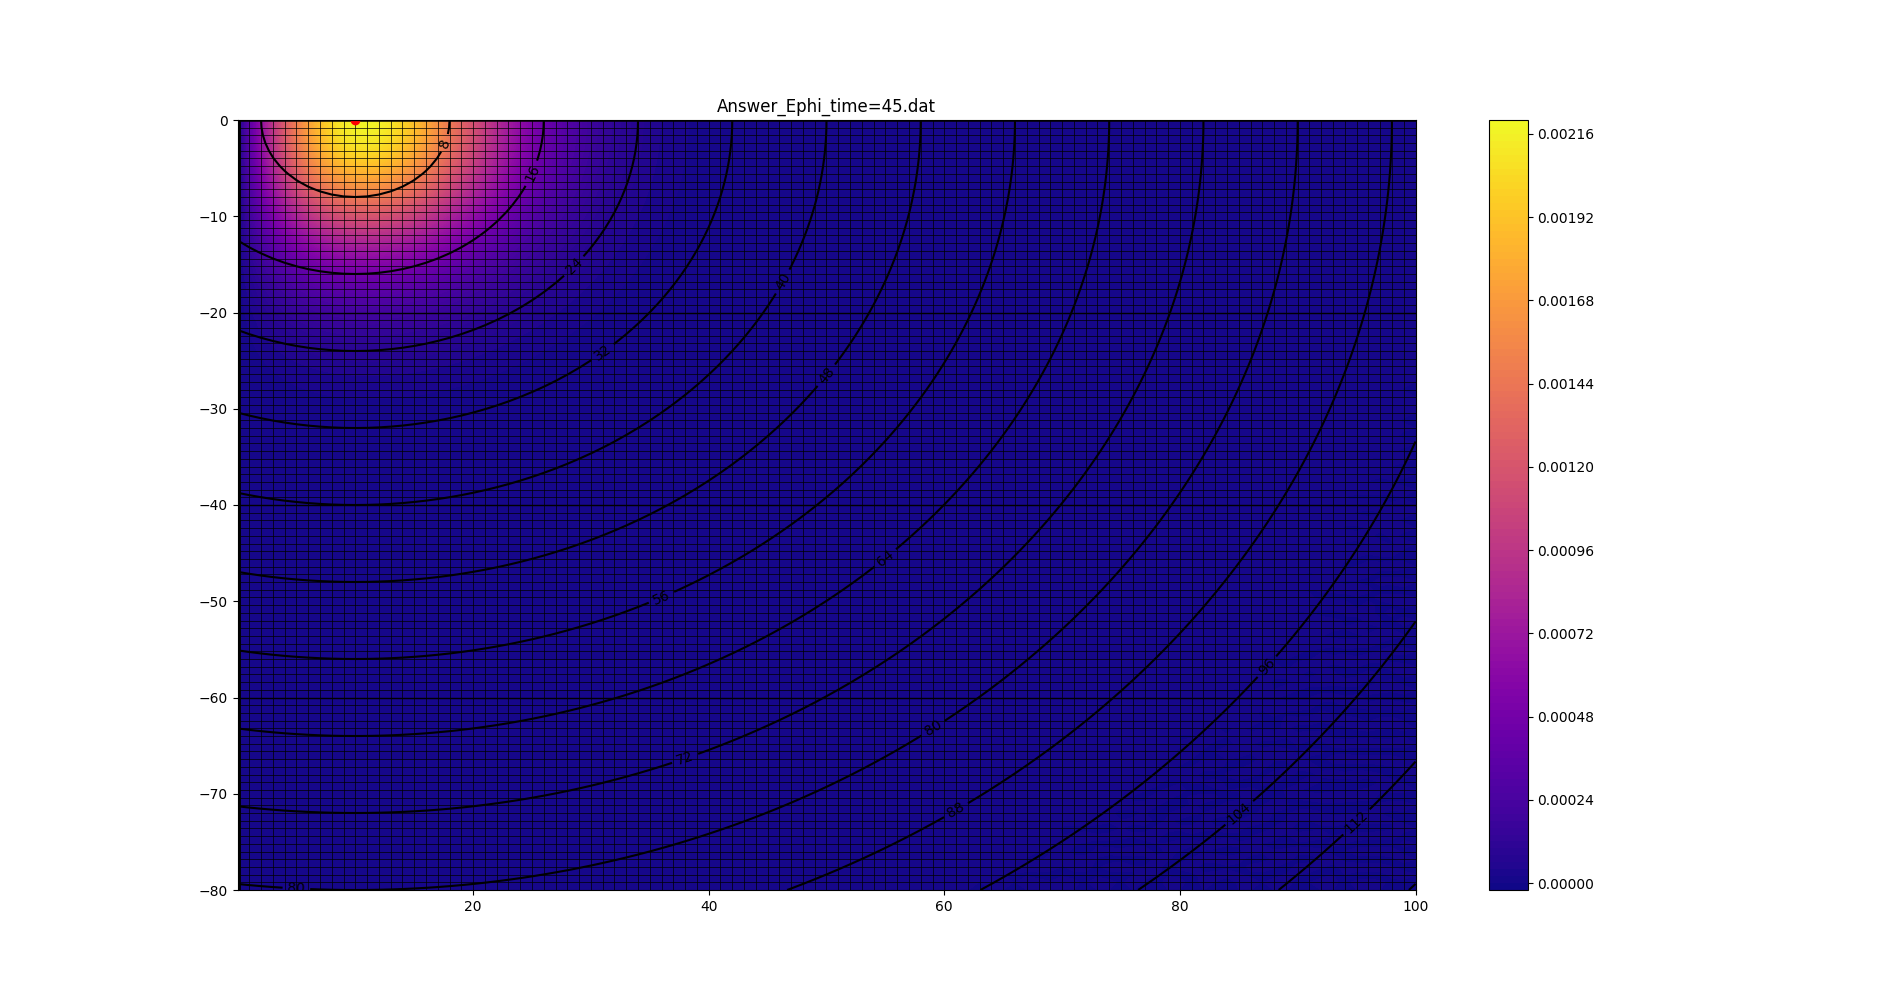
\includegraphics[width=1.0\linewidth]{images/Answer_Ephi_time=45.png}
	\caption{Решение $A_{\varphi}(r, z, 45.0)$}
	\label{fig:E_phi_45}
\end{figure} 


\begin{figure}
	\centering
	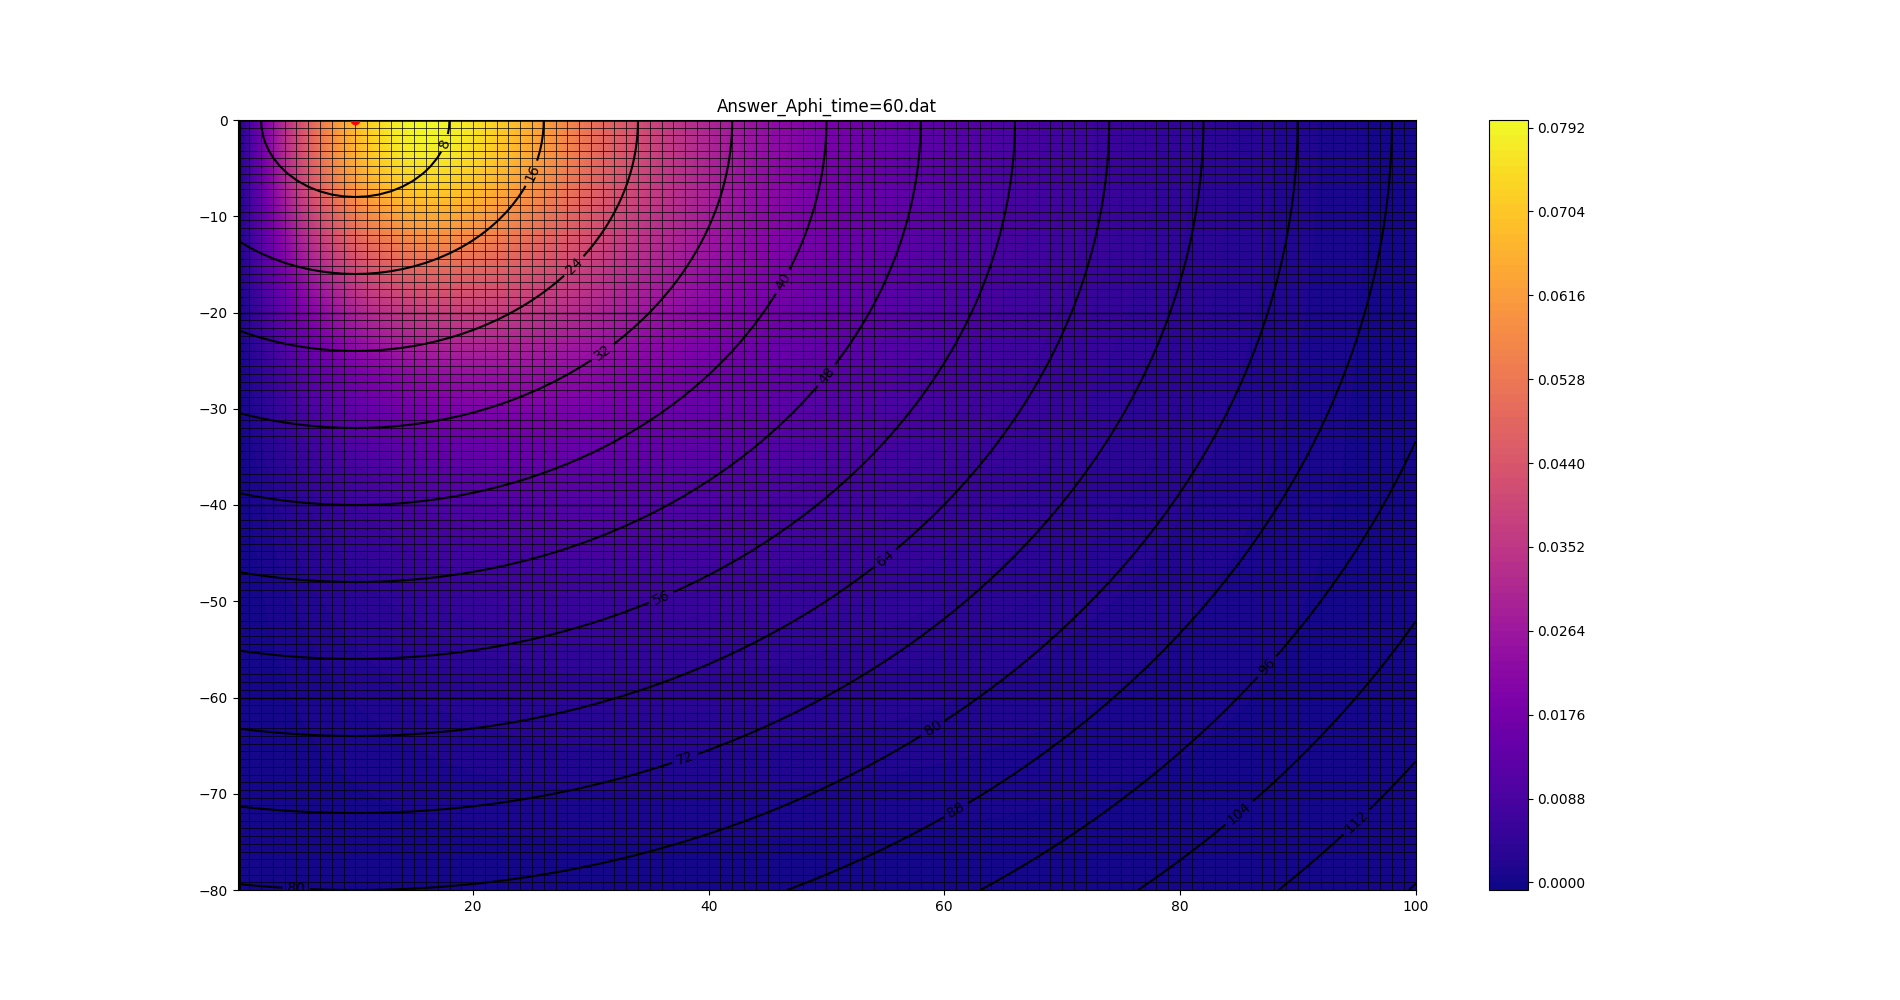
\includegraphics[width=1.0\linewidth]{images/Answer_Aphi_time=60.png}
	\caption{Решение $A_{\varphi}(r, z, 60.0)$}
	\label{fig:A_phi_60}
\end{figure}

\begin{figure}
	\centering
	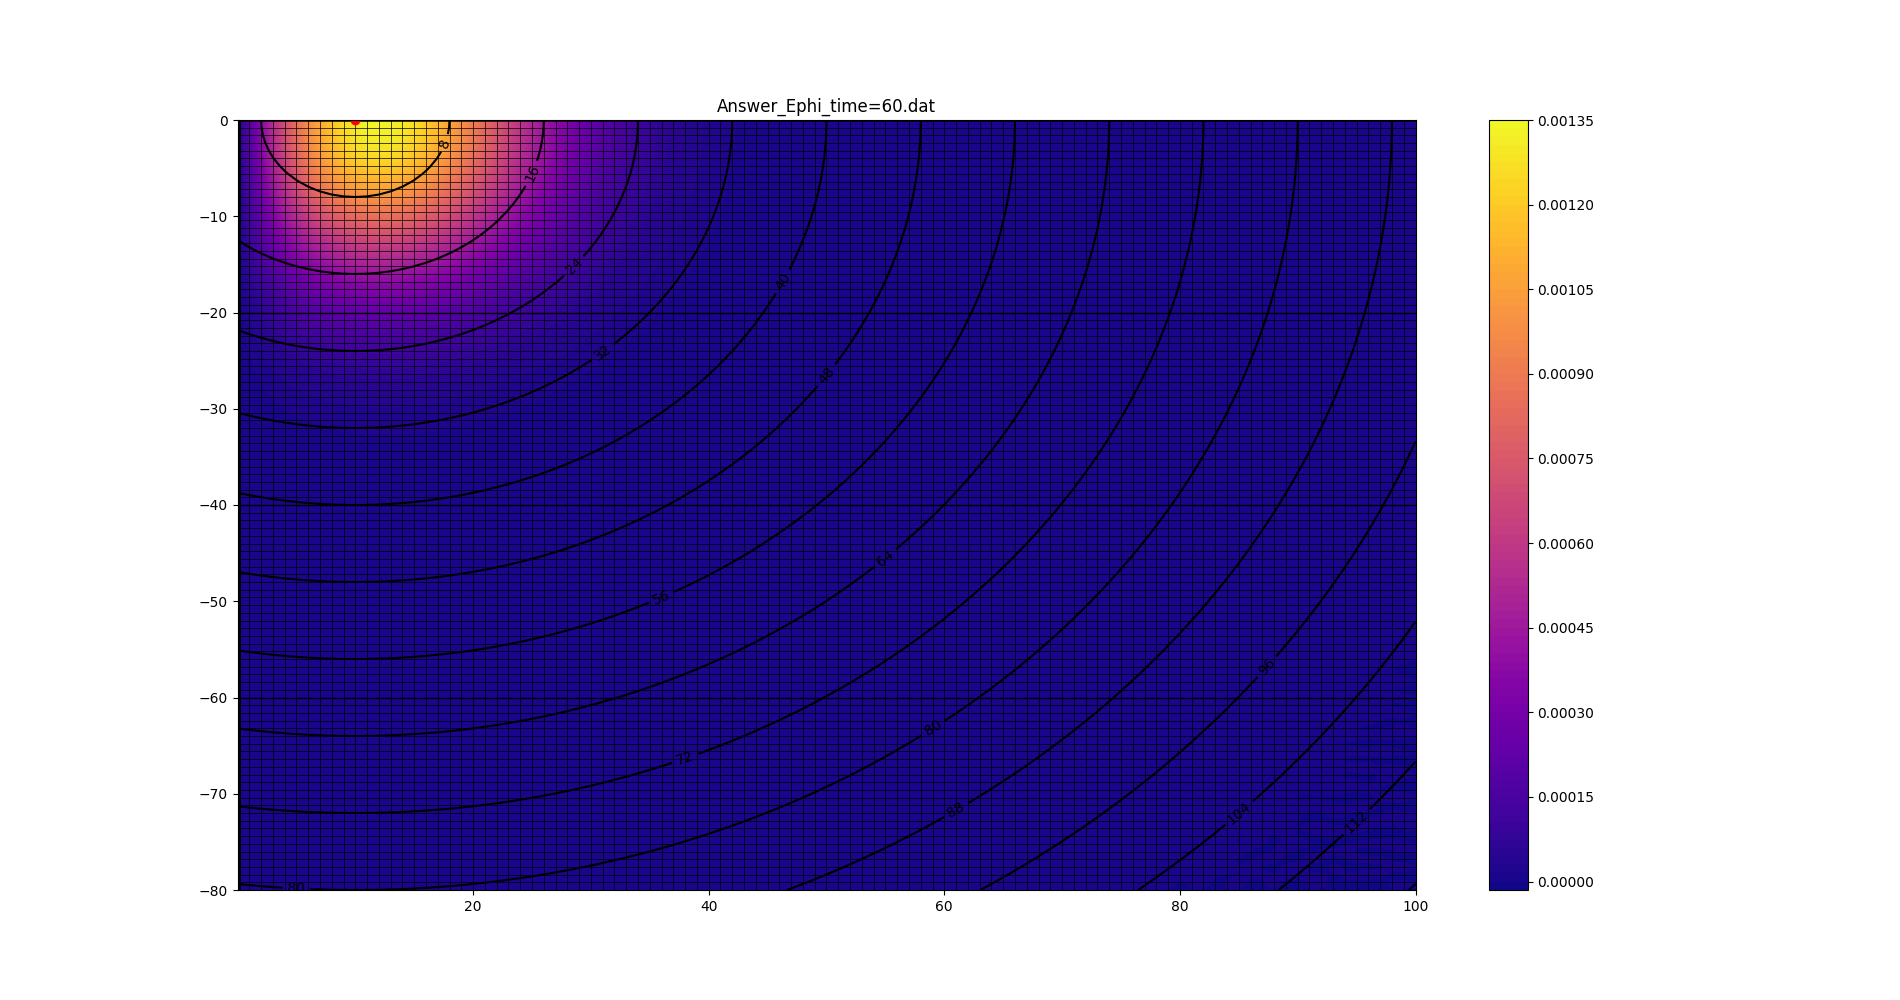
\includegraphics[width=1.0\linewidth]{images/Answer_Ephi_time=60.png}
	\caption{Решение $A_{\varphi}(r, z, 60.0)$}
	\label{fig:E_phi_60}
\end{figure} 